% !TeX root = RJwrapper.tex
\title{echos: An R Package for Automatic Time Series Forecasting using Echo State Networks}


\author{by Alexander Häußer}

\maketitle

\abstract{%
The paper introduces echos, an R package for automatic univariate time series modeling and forecasting using Echo State Networks (ESNs). ESNs represent an efficient and flexible method that combines reservoir computing for dimensionality expansion with a simple linear model estimated via ridge regression. The package provides two complementary interfaces: a base R interface for modeling numeric vectors, integrating seamlessly into traditional R workflows; and a tidy interface, built upon the tsibble and fable frameworks, for streamlined forecasting, evaluation, and visualization in tidyverse-oriented workflows. echos implements lightweight and fully automated procedures, enabling accurate forecasting without extensive hyperparameter tuning or manual configuration. The package's capabilities are illustrated using synthetic and real-world data, accompanied by two case studies. The first case study demonstrates the base R interface, and the second showcases the tidy interface. Both case studies include reproducible coding examples, ensuring users can readily apply ESNs to their forecasting tasks.
}

\section{Introduction}\label{introduction}

Time series forecasting is fundamental in domains such as finance, economics, and energy, where accurate forecasts support decision-making and resource planning. Over the last few decades, various methods for time series forecasting have been developed, ranging from statistical approaches like autoregressive integrated moving average (ARIMA) and exponential smoothing state space models (ETS) to more advanced techniques like machine learning algorithms and neural network models. Neural networks offer a flexible, data-driven approach for modeling linear and nonlinear relationships in time series data. Among the various neural network architectures, recurrent neural networks (RNNs) are particularly well-suited for sequential data due to their ability to process temporal dependencies in the hidden state, making them popular for time series applications.

An interesting variant of RNNs is the echo state network (ESN) \citep{Jaeger2001}, a type of reservoir computing (RC) model. ESNs expand the input signal into a high-dimensional feature space through a fixed, nonlinear reservoir and then use a comparatively simple readout mechanism, often a linear model estimated via ridge regression, to produce forecasts \citep{Lukosevicius2009, Lukosevicius2012}. By decoupling most of the network parameters from backpropagation, ESNs greatly reduce the computational overhead that characterizes many neural network approaches. Moreover, they simplify model building and hyperparameter tuning, making them appealing for large-scale, fully automatic forecasting tasks.

Despite the growing interest in RC and ESNs, there are relatively few mature and well-maintained software implementations available, particularly within R. \pkg{ReservoirPy} \citep{ReservoirPy} is a Python library designed for efficient and flexible implementation of RC architectures, particularly ESNs. It supports both offline and online training, parallel computation, sparse matrix operations, and fast spectral initialization, and includes advanced features such as deep and feedback reservoirs, as well as graphical tools for hyperparameter optimization. \CRANpkg{reservoirnet} is an R package that serves as a wrapper for \pkg{ReservoirPy}, enabling R users to access the full functionality of the Python library through the \CRANpkg{reticulate} \citep{reticulate} interface. It inherits all advanced features of \pkg{ReservoirPy}, including support for complex reservoir architectures, efficient computation, and hyperparameter exploration, while providing integration with R workflows.

In contrast, the R package \CRANpkg{echos} \citep{echos} is a lightweight implementation focused on fast, fully automatic modeling and forecasting of univariate time series using ESNs. Its emphasis is on ease of use and automation: \CRANpkg{echos} requires minimal manual configuration, offers seamless integration with R's time series ecosystem, and is optimized for practitioners seeking rapid and reliable forecasts rather than customizable RC research. Source code and the development version of \CRANpkg{echos} are available in the \href{https://github.com/ahaeusser/echos}{GitHub repository}.

In the R ecosystem for time series forecasting, there is a long-standing tradition of using the \CRANpkg{forecast} package \citep{forecast}, which provides methods for statistical models (e.g., ARIMA, ETS) as well as some neural network approaches. In recent years, an alternative approach has emerged based on the so-called tidy philosophy: the \CRANpkg{fable} package \citep{fable}, along with its supporting packages \CRANpkg{tsibble} \citep{tsibble} and \CRANpkg{fabletools} \citep{fabletools}. Unlike the \texttt{ts} class, which underpins much of the traditional time series functionality in R, \CRANpkg{tsibble} provides a data structure for temporal data that embraces tidy data principles, facilitating both user-friendliness and scalability. A \texttt{tsibble} is a special type of a \texttt{tibble} (or \texttt{data.frame}), specifically designed for time series data. It offers powerful features for time-based indexing, handling irregular time series, and performing group-wise forecasts in a straightforward manner. The \CRANpkg{fable} package builds on \CRANpkg{tsibble} to streamline forecasting workflows, model specification, and forecast reconciliation. This modern tidy approach has proven especially useful for handling datasets with multiple time series, enabling more user-friendly analysis compared to the traditional workflow.

The package \CRANpkg{echos} offers two complementary interfaces:

\begin{enumerate}
\def\labelenumi{\arabic{enumi}.}
\tightlist
\item
  \textbf{Base R interface:} The base approach accepts a \texttt{numeric} vector as input to integrate seamlessly into existing workflows relying on traditional data structures and types. A drawback of the base approach is that modeling multiple time series requires iterating over them explicitly (e.g., \texttt{for}-loops or functions from the \texttt{apply()} or \texttt{map()} family).
\item
  \textbf{Tidy interface:} The tidy approach connects directly to the \CRANpkg{fable} framework based on \CRANpkg{tsibble}, leveraging \CRANpkg{fabletools}. The tidy approach enables streamlined modification, analysis, modeling, and forecasting of multiple series, even if they have different lengths (i.e., varying start and end dates), making the overall workflow more straightforward.
\end{enumerate}

Both interfaces enable fully automatic model building and forecasting using ESNs, minimizing the need for extensive hyperparameter tuning. The \CRANpkg{echos} package aims to make RC methods more accessible to both researchers and practitioners. Table \ref{tab:comparison} summarizes the key differences between \CRANpkg{echos} and \pkg{ReservoirPy} in terms of scope, interface philosophy, and supported forecasting and evaluation functionality.

\begin{longtable}[]{@{}
  >{\raggedright\arraybackslash}p{(\linewidth - 4\tabcolsep) * \real{0.3333}}
  >{\raggedright\arraybackslash}p{(\linewidth - 4\tabcolsep) * \real{0.3333}}
  >{\raggedright\arraybackslash}p{(\linewidth - 4\tabcolsep) * \real{0.3333}}@{}}
\caption{\label{tab:comparison} Comparison between the R package \CRANpkg{echos} and the Python library \pkg{ReservoirPy}, highlighting differences in scope, interface philosophy, tuning workflows, forecasting features, uncertainty quantification, and distribution.}\tabularnewline
\toprule\noalign{}
\begin{minipage}[b]{\linewidth}\raggedright
\textbf{Dimension}
\end{minipage} & \begin{minipage}[b]{\linewidth}\raggedright
\CRANpkg{echos}
\end{minipage} & \begin{minipage}[b]{\linewidth}\raggedright
\pkg{ReservoirPy}
\end{minipage} \\
\midrule\noalign{}
\endfirsthead
\toprule\noalign{}
\begin{minipage}[b]{\linewidth}\raggedright
\textbf{Dimension}
\end{minipage} & \begin{minipage}[b]{\linewidth}\raggedright
\CRANpkg{echos}
\end{minipage} & \begin{minipage}[b]{\linewidth}\raggedright
\pkg{ReservoirPy}
\end{minipage} \\
\midrule\noalign{}
\endhead
\bottomrule\noalign{}
\endlastfoot
Primary scope & End-to-end ESN time series forecasting & General RC/ESN framework \\
Interface philosophy & High-level interface via base R and \CRANpkg{fable}/\CRANpkg{tsibble} ecosystem & Modular nodes and models via the \pkg{NumPy}/\pkg{SciPy} ecosystem \\
Model selection and tuning & Automated training, tuning, and time series cross-validation & Hyperparameter tools available; tuning and validation are user-assembled \\
Forecasting strategy & Built-in recursive multi-step forecasting & Multi-step forecasting implemented by the user \\
Multivariate and exogenous inputs & Primary focus on univariate forecasting & Multivariate and exogenous inputs supported \\
Uncertainty quantification & Forecast intervals via simulation using a moving block bootstrap of residuals & No dedicated interval interface; uncertainty typically implemented by the user \\
Data preprocessing and pipeline & Data preprocessing, reservoir generation, and estimation are handled automatically & Data preparation is typically explicit; inputs are provided as arrays \\
Diagnostics and evaluation & Built-in evaluation and plotting methods & Evaluation typically performed with external tooling \\
Performance & Uses compiled components via \CRANpkg{Rcpp}/\CRANpkg{RcppArmadillo} & Relies on \pkg{NumPy}/\pkg{SciPy}, supports sparse matrices and parallel computation \\
License and distribution & GPL-3; distributed on CRAN & MIT; distributed on PyPI \\
\end{longtable}

The remainder of this paper is structured as follows: Section 2 covers the underlying methodology for applying ESNs in time series forecasting. Section 3 provides an overview of the available functions and methods as well as details on the implementation of the algorithm, from data preprocessing and reservoir generation to model estimation and selection. Section 4 shows illustrative examples of synthetic and real-world time series data and demonstrates the pattern recognition and learning capabilities of the proposed approach. Section 5 presents two case studies, one using base R and another using tidy R, to demonstrate the package's capabilities in real-world forecasting tasks. Finally, Section 6 summarizes the main findings.

\section{Basic model}\label{basic-model}

ESNs are an RC technique, and compared to other neural networks, they are similar in architecture but different in training. This approach leads to a fast, simple, and constructive supervised learning algorithm for neural networks. ESNs make a conceptual and computational separation between the hidden layer (dynamic reservoir as a nonlinear temporal dimensionality expansion) and a recurrence-free (usually linear) readout that produces the desired output from the expansion. This separation is based on the understanding that the input is expanded into a rich enough reservoir state space. These so-called internal states are combined into the desired output. The traditional training methods for RNNs often do not make a conceptual separation between the input, hidden, and output layers, where all the weights within a neural network are trained simultaneously \citep{Lukosevicius2009}.

The architecture of an ESN is similar to other neural networks: an input layer, a hidden layer, and an output layer. The idea of an ESN is the application of a large random reservoir (e.g., 100 units) as a source of the dynamic behavior of the network, from which the internal states are combined into the required output. Depending on the application, the reservoir size can be substantially larger. Unlike other neural networks, only the weights from the hidden layer to the output layer \(\mathbf{W}^\mathrm{out}\) are trained, while the input weights \(\mathbf{W}^\mathrm{in}\) (input-to-hidden connections) and the reservoir weights \(\mathbf{W}\) (hidden-to-hidden connections) are randomly initialized and fixed \citep{Lukosevicius2012}. Figure \ref{fig:esn-architecture} provides a schematic overview of the basic ESN architecture.

Formally, consider a univariate, (weak-) stationary time series \(\{y_t\}_{t=1}^{T}\). An ESN maps an input \(u_t\) (e.g., \(y_{t-1}\)) into a set of internal states, denoted by a vector \(\mathbf{x}_t = (x_{1,t}, x_{2,t}, \ldots, x_{N_x, t})^\top\), where \(N_x\) is the number of reservoir units. There is a distinction between non-leaky and leaky ESNs. In a non-leaky ESN, the reservoir state is replaced at each time step by the newly computed nonlinear update. In a leaky ESN (leaky-integrator), the state update includes an additional smoothing (integration) step, so the new state becomes a blend of the previous state and the newly computed update. For a standard non-leaky ESN, the reservoir update \(\tilde{\mathbf{x}}_t\) is computed via

\begin{equation}
\tilde{\mathbf{x}}_t = \tanh\!\left(\mathbf{W}^{\mathrm{in}}\,u_t + \mathbf{W}\,\mathbf{x}_{t-1}\right), \quad t = 1, 2, \ldots, T,
\label{eq:reservoir}
\end{equation}

where \(\mathbf{x}_0 = \mathbf{0}\) is the initial state and \(\tanh(\cdot)\) is the hyperbolic tangent activation function applied element-wise. Functions other than the hyperbolic tangent can also be used as the activation function. However, it is the most common choice in practice. The hidden-to-hidden (reservoir) connections are encoded in a matrix \(\mathbf{W}\in\mathbb{R}^{N_x \times N_x}\), while the input-to-hidden connections are encoded in \(\mathbf{W}^{\mathrm{in}}\in\mathbb{R}^{N_x \times N_u}\), where \(N_u\) is the dimension of the input (e.g., \(N_u = 1\) for a single-input unit \(y_{t-1}\)).

The input weight matrix \(\mathbf{W}^{\mathrm{in}}\) and the reservoir weight matrix \(\mathbf{W}\) are generated randomly, i.e., both matrices are populated with random numbers, usually drawn from a uniform distribution. Nevertheless, other distributions are possible, like the normal distribution. Both matrices remain fixed after random initialization. For a leaky integrator ESN, a leakage rate \(\alpha \in (0,1]\) can additionally be introduced:

\begin{equation}
\mathbf{x}_t = (1 - \alpha)\,\mathbf{x}_{t-1} + \alpha \tilde{\mathbf{x}}_t.
\label{eq:leaky-reservoir}
\end{equation}

The hidden state update then becomes a blend of the old internal state and the newly computed nonlinear transformation, thus providing a form of memory, similar to exponential smoothing applied to the internal states. \(\alpha = 1\) recovers the non-leaky ESN, where each new reservoir state fully replaces the old one. \(0 < \alpha < 1\) yields a weighted average between \(\mathbf{x}_{t-1}\) and the \(\tanh(\cdot)\) term, effectively slowing down changes in the reservoir states and allowing the ESN to capture longer-term dependencies \citep{Lukosevicius2012}.

A further hyperparameter within an ESN is the spectral radius of the reservoir weight matrix, i.e., the maximum absolute eigenvalue of this matrix. Rescaling \(\mathbf{W}_1 = {|\max(\lambda (\mathbf{W}_0))|}^{-1} \mathbf{W}_0\) to a matrix with unit spectral radius and scaling \(\mathbf{W}_1\) by the ultimate spectral radius \(\rho\) gives the final reservoir weight matrix \(\mathbf{W} = \rho \mathbf{W}_1\). Scaling the reservoir weight matrix to a spectral radius \(\rho\) changes the width of the distribution of its elements. For an ESN to function correctly, it needs to satisfy the so-called echo state property, which ensures that the influence of previous inputs fades over time. This means the current state of the reservoir should be a reflection of recent inputs rather than distant past inputs. The spectral radius helps to ensure this property. If the spectral radius is too large (greater than 1), the states in the reservoir might not fade away but instead could grow without bound, leading to instability. If it is too small, the states might fade too quickly, losing important information. A spectral radius close to 1 means that the network can maintain a memory of past inputs for a longer time, which is often desirable \citep{Lukosevicius2012}.

The internal states are computed according to equations \eqref{eq:reservoir} and \eqref{eq:leaky-reservoir} and, together with an intercept term, stacked over time into the design matrix \(\mathbf{X}\), whose rows are of the form \((1,  x_{1,t}, x_{2,t}, ..., x_{N_x, t})\). Hence, the first column of \(\mathbf{X}\) is an intercept of ones, and the remaining columns contain the reservoir states over time. Note that the typical initial values \(\mathbf{x}_{0} = 0\) often introduce an unnatural starting point of the internal states (initial transient). Discarding these initial time steps is advisable until the reservoir has warmed up. The number of time steps to discard from the design matrix depends on the time series and reservoir parameters \citep{Lukosevicius2012}. For a univariate response time series \(\{y_t\}_{t=1}^T\) (equivalently, a single-output setting with \(N_y = 1\)), the linear model can be written as:

\begin{equation}
\mathbf{y} = \mathbf{X}\,\mathbf{W}^{\mathrm{out}}\;+\;\boldsymbol{\epsilon},
\label{eq:linear-model}
\end{equation}

where \(\mathbf{W}^{\mathrm{out}} \in \mathbb{R}^{(N_x+1) \times 1}\) are the readout weights to be estimated and \(\boldsymbol{\epsilon}\) is an error term with \(\mathbb{E}[\boldsymbol{\epsilon}]=\mathbf{0}\). A common issue for ESNs is overfitting, which occurs when a model is built that captures the signal and noise in the data. The task is to create a stable model that generalizes well while forecasting. Hence, mechanisms are required to mitigate overfitting and reduce prediction errors. In the original literature \citep{Jaeger2001, Jaeger2002}, ridge regression is used to train a linear model. With many highly correlated features, linear models estimated via ordinary least squares (OLS) can suffer from multicollinearity, leading to unstable estimates, overfitting, and poor forecasts. Ridge regression can reduce or eliminate these effects. Alternative approaches for model estimation in the existing literature are LASSO (least absolute shrinkage and selection operator) and Elastic-Net \citep{Ceperic2014, Qiao2019, Xu2016}.

\begin{figure}

{\centering 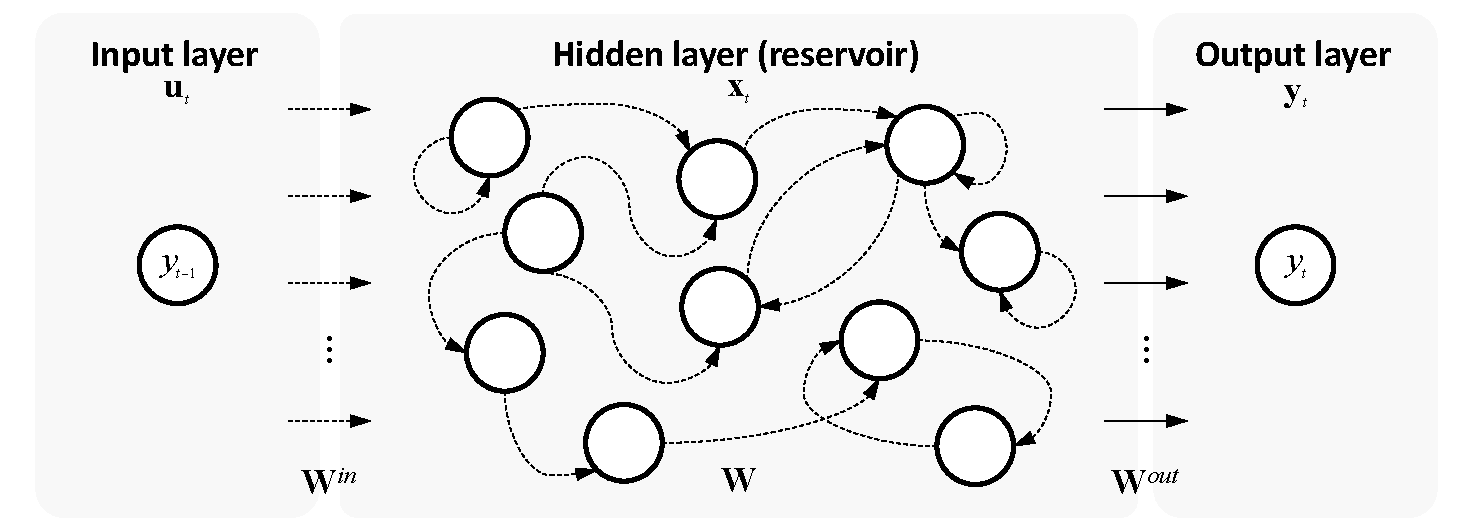
\includegraphics[width=1\linewidth]{figures/figure_01_esn_architecture} 

}

\caption{Basic ESN architecture with an input layer $\mathbf{u}_{t}$, a hidden layer (reservoir) $\mathbf{x}_{t}$ and an output layer $\mathbf{y}_{t}$. The figure illustrates the univariate first-order autoregressive case, where the single input is the lagged observation $y_{t-1}$ and the single output is $y_t$. Dashed lines indicate fixed, random weights, i.e., input weights $\mathbf{W}^\mathrm{in}$ and reservoir weights $\mathbf{W}$. Solid lines indicate trainable output weights $\mathbf{W}^\mathrm{out}$.}\label{fig:esn-architecture}
\end{figure}

\section{Implementation}\label{implementation}

ESNs in the \CRANpkg{echos} package can be trained and used for forecasting through two complementary sets of functions: a base R interface and a tidy interface built on top of the \CRANpkg{fable} framework and the \CRANpkg{tsibble} data structure. By separating these interfaces, the package provides both flexibility and usability as standalone functions and a streamlined pipeline that leverages tidy data principles \citep{tidyverse}. Table \ref{tab:functions} gives an overview of the functions, methods, and datasets available.

\begin{longtable}[]{@{}
  >{\raggedright\arraybackslash}p{(\linewidth - 2\tabcolsep) * \real{0.2479}}
  >{\raggedright\arraybackslash}p{(\linewidth - 2\tabcolsep) * \real{0.7521}}@{}}
\caption{\label{tab:functions} Overview of the functions and methods for model training, forecasting, evaluation, and visualization as well as the built-in datasets.}\tabularnewline
\toprule\noalign{}
\begin{minipage}[b]{\linewidth}\raggedright
\textbf{Function}
\end{minipage} & \begin{minipage}[b]{\linewidth}\raggedright
\textbf{Description}
\end{minipage} \\
\midrule\noalign{}
\endfirsthead
\toprule\noalign{}
\begin{minipage}[b]{\linewidth}\raggedright
\textbf{Function}
\end{minipage} & \begin{minipage}[b]{\linewidth}\raggedright
\textbf{Description}
\end{minipage} \\
\midrule\noalign{}
\endhead
\bottomrule\noalign{}
\endlastfoot
\textbf{Base functions} & \\
\(~~~\) \texttt{train\_esn()} & Train an ESN on a univariate time series \\
\(~~~\) \texttt{forecast\_esn()} & Forecast a trained ESN \\
\(~~~\) \texttt{tune\_esn()} & Tune hyperparameters of an ESN \\
\(~~~\) \texttt{print.esn()} & Print model specification \\
\(~~~\) \texttt{summary.esn()} & Provide a detailed summary \\
\(~~~\) \texttt{summary.tune\_esn()} & Provide a summary of the hyperparameter tuning \\
\(~~~\) \texttt{is.esn()} & Checks if the object is of class \texttt{esn} \\
\(~~~\) \texttt{is.forecast\_esn()} & Checks if the object is of class \texttt{forecast\_esn} \\
\(~~~\) \texttt{is.tune\_esn()} & Checks if the object is of class \texttt{tune\_esn} \\
\(~~~\) \texttt{plot.esn()} & Plot internal states of a trained ESN model \\
\(~~~\) \texttt{plot.forecast\_esn()} & Plot \texttt{point} and \texttt{interval} forecasts, \texttt{actual} and \texttt{fitted} values \\
\(~~~\) \texttt{plot.tune\_esn()} & Plot forecasts from a tuned ESN object \\
\(~~~\) \texttt{run\_reservoir()} & Create the reservoir, i.e., the internal states \\
\textbf{Tidy functions} & \\
\(~~~\) \texttt{ESN()} & Train an ESN on tidy time series data \\
\(~~~\) \texttt{forecast.ESN()} & Forecast a trained ESN \\
\(~~~\) \texttt{fitted.ESN()} & Extract fitted values from a trained ESN \\
\(~~~\) \texttt{residuals.ESN()} & Extract residuals from a trained ESN \\
\(~~~\) \texttt{model\_sum.ESN()} & Print model specification \\
\(~~~\) \texttt{tidy.ESN()} & Extract estimated coefficients \\
\(~~~\) \texttt{glance.ESN()} & Summary statistics during random search \\
\(~~~\) \texttt{report.ESN()} & Provide a detailed summary \\
\(~~~\) \texttt{filter\_esn()} & Filter ESN models from \texttt{mdl\_df} (mable) \\
\(~~~\) \texttt{reservoir()} & Return the reservoir from a trained ESN as a \texttt{tibble} \\
\textbf{Datasets} & \\
\(~~~\) \texttt{m4\_monthly\_subset} & \texttt{tsibble} with six monthly time series \\
\(~~~\) \texttt{synthetic\_data} & \texttt{tibble} with ten synthetic time series \\
\end{longtable}

\subsection{Core functions}\label{core-functions}

The core function \texttt{train\_esn()} performs end-to-end training of an ESN model. It takes a \texttt{numeric} vector representing a univariate time series \texttt{y} as input and internally manages data preprocessing, reservoir generation, and model estimation and selection. Arguments with a default value of \texttt{NULL} are handled internally by heuristics or tuned automatically.

The default hyperparameter settings in \texttt{train\_esn()} were chosen to reflect commonly recommended values and practical ranges reported in the ESN literature. In particular, the defaults follow established guidelines on leakage, spectral radius scaling for stable reservoir dynamics, and typical choices for reservoir size and sparsity, providing a robust starting point for automatic forecasting. Overall, these defaults are intended to be conservative and broadly applicable, while remaining consistent with ranges that have been found effective in prior studies \citep{Viehweg2023, Lukosevicius2012}.

\begin{verbatim}
train_esn(
  y,
  lags = 1,
  inf_crit = "bic",
  n_diff = NULL,
  n_states = NULL,
  n_models = NULL,
  n_initial = NULL,
  n_seed = 42,
  alpha = 1,
  rho = 1,
  tau = 0.4,
  density = 0.5,
  lambda = c(1e-04, 2),
  scale_win = 0.5,
  scale_wres = 0.5,
  scale_inputs = c(-0.5, 0.5)
  )
\end{verbatim}

The input data \texttt{y} must be preprocessed before training and forecasting, as is common with many neural networks. Most time series exhibit nonstationarity due to trends, seasonality, or heteroscedasticity, with trends being especially problematic for ESNs due to the activation function and the resulting reservoir dynamics. Therefore, the Kwiatkowski--Phillips--Schmidt--Shin (KPSS) test \citep{Kwiatkowski1992} is employed to assess the stationarity of the output variable \(y_t\). If the series is nonstationary, first differences (\(z_t = y_t - y_{t-1}\)) are calculated to stabilize the mean of the time series by removing changes in the level, thus reducing or eliminating trends \citep{Hyndman2021}. In \CRANpkg{echos}, differencing is handled as a lightweight preprocessing step aimed at reducing nonseasonal nonstationarity prior to reservoir generation. Concretely, the number of differences \texttt{n\_diff} is determined by applying a KPSS test for level stationarity and, if the null is rejected, applying a single first difference to mitigate level/trend effects that can be problematic for ESN reservoir dynamics. This procedure is intentionally conservative and does not attempt automatic seasonality detection or seasonal differencing (e.g., via \texttt{forecast::nsdiffs()}). For strongly seasonal series, seasonal adjustment or seasonal differencing is therefore recommended as an upstream preprocessing step using established tooling in the \CRANpkg{forecast} or \CRANpkg{fable} ecosystem before calling \texttt{train\_esn()} or \texttt{ESN()}.

After detrending, the output variable is scaled to the interval \([a, b]\) by

\begin{equation}
z_{t}' = a + \frac{(z_t - \min(z_t))(b-a)}{\max(z_t)-\min(z_t)},
\label{eq:scaling}
\end{equation}

where \(a\) is the lower limit and \(b\) is the upper limit for the new scale of the time series. Empirical research indicates good results when scaling inputs to the symmetric interval \([-0.5, 0.5]\). Other scaling methods, such as min-max or standardization (z-score normalization) could also be used, but are not implemented. For simplicity, \(y_t\) (or matrix notation \(\mathbf{y}\)) is used in the following, assuming input data is already preprocessed. After training and forecasting, fitted values and forecasts are inversely differenced and rescaled back to the original scale.

Key arguments of \texttt{train\_esn()} are defined as follows: Differencing (\texttt{n\_diff}) specifies the number of differences to remove nonstationarity, automatically determined via KPSS if set to \texttt{NULL}. After differencing, input scaling (\texttt{scale\_inputs}) stabilizes the input data in the interval \([-0.5, 0.5]\). Embedding (\texttt{lags}) defaults to 1, meaning the first autoregressive lag is used as input (\(u_t = y_{t-1}\)).

The reservoir generation phase involves several hyperparameters and the internal states are calculated according to equations \eqref{eq:reservoir} and \eqref{eq:leaky-reservoir}. By default, the number of internal states \texttt{n\_states} is determined by the following simple heuristic: \(N_x = \min(\lfloor \tau T \rfloor, 200)\), where \(T\) is the length of the time series and \(\tau\) is the so-called reservoir scaling parameter to dynamically control the reservoir size. The default is \(\tau = 0.4\), i.e., the number of internal states is set to 40\% of the number of observations \(T\) of the time series. To ensure that the output is an integer value, the floor function \(\lfloor \cdot \rfloor\) is applied, rounding the output down to the nearest integer. Additionally, the value is capped at 200 to limit the reservoir size for long time series. This heuristic is an implementation choice intended to provide a simple, data-adaptive default that balances model flexibility and runtime; it should be understood as a reasonable starting point rather than a theoretically optimal rule, and users can override \texttt{n\_states} (or tune \texttt{tau} if required).

The input weight matrix \(\mathbf{W^\mathrm{in}}\) is a dense matrix populated with random numbers (i.e., fully connected), drawn from a uniform distribution, where the interval is defined by \texttt{scale\_win}, defaulting to \([-0.5, 0.5]\). The (initial) reservoir weight matrix \(\mathbf{W}\) is a (structurally) sparse matrix with random numbers, drawn from a uniform distribution, where the interval is defined by \texttt{scale\_wres}. By default, the reservoir weight matrix has a \texttt{density} of 50\%, i.e., half of the matrix elements are (randomly) padded with random numbers, while the other half is filled with zeros. This approach ensures that the reservoir remains well-connected while avoiding a fully dense weight matrix. The spectral radius (\texttt{rho}) defaults to 1, balancing retaining memory of past inputs and ensuring the stability of the network. Leaky integration (\texttt{alpha}) defaults to 1 (non-leaky), but values between 0 and 1 can blend past and current information to enhance memory. Finally, a warm-up period (\texttt{n\_initial}) discards the initial 5\% of internal states by default to reduce transient effects.

For model estimation and selection, ridge regression is employed to mitigate overfitting due to the typically large reservoir and correlated internal states. The ridge regression estimator for the linear model in equation \eqref{eq:linear-model} has a closed-form solution:

\begin{equation}
\mathbf{\widehat{W}}^\mathrm{out} = \left(\mathbf{X}^\top \mathbf{X} + \mathbf{R}_{\lambda}\right)^{-1}\mathbf{X}^\top\mathbf{y},
\label{eq:estimator}
\end{equation}

where \(\mathbf{R}_{\lambda} = diag(0, \lambda, ..., \lambda)\) is the regularization matrix. The \(0\) in the diagonal matrix ensures that the intercept term is untouched by the regularization, while the other \(N_x\) coefficients are penalized with a common penalty \(\lambda\). The regularization matrix is added along the diagonal of \(\mathbf{X}^{\top}\mathbf{X}\) before inversion. If the predictor variables in the design matrix are highly correlated with each other, which is almost always the case within an ESN if the reservoir is large enough, then the matrix \(\mathbf{X}\) does not have full rank and \(\mathbf{X}^{\top}\mathbf{X}\) is not invertible. There is no unique solution to the linear regression problem. Adding the small term \(\lambda\) along the diagonal of \(\mathbf{X}^{\top}\mathbf{X}\) makes all columns linearly independent; hence the matrix \((\mathbf{X}^{\top}\mathbf{X} + \mathbf{R}_{\lambda})\) is invertible.

Ridge regression navigates the bias-variance trade-off by penalizing large coefficients, balancing goodness-of-fit and complexity. Ridge regression penalizes the coefficients such that less influential internal states are more strongly shrunk toward zero. For \(\lambda = 0\), the estimator in \eqref{eq:estimator} is equal to OLS, and for \(\lambda \rightarrow \infty\), all coefficients are zero (except the coefficient for the intercept term). For \(\lambda\) in between, the two ideas are balanced: goodness-of-fit and shrinking coefficients towards zero, thereby introducing bias but reducing the estimate's variance \citep{Hastie2009}.

Now that the estimation method is defined, a disciplined way to determine the regularization parameter \(\lambda\) is required. A simple but effective approach is to search different values for the regularization parameter and choose the value that results in a model that achieves the best performance on a given time series. The best performance here implies a model with high goodness-of-fit but at the same time low model complexity to avoid overfitting (parsimonious model).

A popular strategy is to choose the regularization parameter \(\lambda\) by information criteria \citep{Burnham2002, Hastie2009}. Information criteria measure the balance between model fit and model complexity. By default, \texttt{train\_esn()} uses the Bayesian Information Criterion (BIC) \citep{Schwarz1978}, but other information criteria like the Akaike Information Criterion (AIC) \citep{Akaike1974} or the Hannan-Quinn Criterion (HQC) \citep{Hannan1979} are also implemented. Information criteria measure model fit by the maximum value of the log-likelihood function, while the number of parameters measures model complexity. The number of model parameters in OLS regression corresponds to the number of predictor variables in the model or, equivalently, to the degrees of freedom consumed by the model, which is equivalent to the trace of the projection matrix (hat matrix).

For ridge regression, it is natural to define model complexity analogously by the effective degree of freedom (or effective number of parameters). The trace of the hat matrix \(\mathbf{H}_\lambda\) gives the effective degrees of freedom of the ridge regression:

\begin{equation}
df_{\lambda} = tr\left(\mathbf{H}_\lambda\right) = tr\left({\mathbf{X}{{({\mathbf{X}^{\top}\mathbf{X} + \mathbf{R}_{\lambda}})}^{ - 1}}\mathbf{X}^{\top}}\right).
\label{eq:dof}
\end{equation}

The effective degrees of freedom is a monotone decreasing function of \(\lambda\). Usually, in a linear regression fit with \(N_x\) variables, the degrees of freedom of the fit is \(N_x\), the number of free parameters. The idea is that although all \(N_x\) coefficients in a ridge fit will be non-zero, they are fit in a restricted fashion controlled by \(\lambda\). Note that \(df_{\lambda} = N_x\) when \(\lambda = 0\) (no regularization) and \(df_{\lambda} = 1\) as \(\lambda \rightarrow \infty\), i.e., all coefficients are shrunk towards zero except for the intercept term \citep{Hastie2009}. For the ESN readout in \CRANpkg{echos}, \(\mathbf{X}\) contains \(N_x\) reservoir states plus an intercept, so the reported \texttt{df} lies in \(1 \le df \le N_x+1\).

For example, the BIC can be calculated for a given value of the regularization parameter \(\lambda\) as follows:

\begin{equation}
BIC_{\lambda} = -2 L + \ln(T) df_{\lambda},
\label{eq:bic}
\end{equation}

where \(L\) is the maximum value of the log-likelihood function, \(T\) is the number of observations and \(df_{\lambda}\) are the effective degrees of freedom.

Different optimization algorithms may be used to tune the regularization parameter. However, two of the simplest and most common methods in the machine learning literature are grid search and random search \citep{Bergstra2012}. Grid search defines a search space as a grid of hyperparameter values and evaluates every position in the grid. In contrast, random search defines a search space as a bounded domain of hyperparameter values and randomly samples points in that domain. Usually, the values are sampled from a uniform distribution within a lower and an upper limit.

\citet{Bergstra2012} show empirically and theoretically that random search is more efficient for hyperparameter optimization than grid search. They demonstrate that random search over the same domain can find models that are as good or better within a small fraction of the computational time. Furthermore, random search has the same practical advantages as grid search, e.g., ease of implementation and trivial parallelism.

The function \texttt{train\_esn()} uses random search to optimize the regularization parameter \(\lambda\). By default, the number of candidate models \texttt{n\_models} during the random search is defined internally as \(K = 2N_x\), i.e., the value for \(K\) is double the reservoir size \(N_x\) (\texttt{n\_models\ =\ 2*n\_states}), because the larger the reservoir size, the larger the search space for the regularization parameter should be. Thus, setting \texttt{n\_models} proportional to \texttt{n\_states} provides a simple, budgeted default that increases the random search effort as model capacity grows, while keeping computational cost within a reasonable range; users can increase or decrease \texttt{n\_models} depending on the trade-off between accuracy and runtime. The values for \texttt{lambda} are drawn from a uniform distribution \([10^{-4}, 2]\). The limits were determined through trial and error and yielded favorable results in practice. The candidate models are estimated for all the random \(\lambda\) values, and the corresponding information criteria are calculated. Afterward, the models are ranked, and the model with the minimum information criterion is selected.

To ensure reproducibility, randomization is controlled by a fixed seed (\texttt{n\_seed}). Internally, \texttt{train\_esn()} relies on the function \texttt{run\_reservoir()} written in C++ using \CRANpkg{Rcpp} \citep{Rcpp} and \CRANpkg{RcppArmadillo} \citep{RcppArmadillo}, significantly accelerating reservoir state computations compared to pure R implementations, especially for long time series.

After fitting, \texttt{train\_esn()} returns an object of class \texttt{esn}, including fitted values, internal states, model diagnostics, etc. Once an ESN model is trained, \texttt{forecast\_esn()} can be used to generate forecasts over a user-defined forecast horizon (\texttt{n\_ahead}).

\begin{verbatim}
forecast_esn(
 object, 
 n_ahead = 18,
 levels = c(80, 95),
 n_sim = 100,
 n_seed = 42
)
\end{verbatim}

The implemented approach for generating point forecasts is recursive forecasting: rather than predicting the entire forecast horizon \(h\) in a single step, the network generates each successive forecast based on the most recent data, including its own predictions. Specifically, after estimating the one-step ahead forecast \(\hat{y}_{T+1 \mid T}\) (with information up to time \(T\)), it is treated as the new input \(u_{T+1} = \hat{y}_{T+1 \mid T}\). The reservoir is updated accordingly to produce \(\hat{y}_{T+2 \mid T}\) (two-step ahead forecast with information up to time \(T\)), and so forth, until the desired forecast horizon \(h\) is reached. This scheme effectively transforms the ESN into an autoregressive-like system, where each new forecast depends on previous forecasts once real observations are no longer available. While recursive forecasting can accumulate errors over multiple steps, it remains a straightforward and commonly used forecasting strategy \citep{BenTaieb2014}.

To quantify forecast uncertainty, future sample paths are simulated via a moving block bootstrap based on the (in-sample) residuals and the empirical quantiles of the distribution are estimated. A moving block bootstrap is used because resampling contiguous residual blocks preserves short-range serial dependence, unlike an i.i.d. residual bootstrap \citep{Kunsch1989}. The residual series \(\epsilon_t\) is centered and resampled into contiguous blocks using a block length \(\ell = \lfloor T^{1/3} \rfloor\), where \(T\) is the number of residuals. Choosing \(\ell\) involves a bias--variance trade-off: larger blocks preserve more serial dependence but reduce the number of effectively independent resampled blocks. The rule \(\ell = \lfloor T^{1/3} \rfloor\) is a widely used default, consistent with theoretical results that suggest block lengths that are optimal in terms of mean squared error for block bootstrap procedures \citep{Politis1994, Politis2004}. For each simulated path, blocks are drawn repeatedly with replacement until their total length reaches the forecast horizon \(h\). The selected blocks are concatenated in the order they are drawn, and any excess observations beyond the forecast horizon are discarded. This residual-based bootstrap assumes that the centered residual series is approximately weakly stationary. If residual diagnostics indicate remaining structure (e.g., strong autocorrelation or conditional heteroscedasticity), the resulting intervals may be miscalibrated and should be interpreted with caution.

Each sequence is added to the corresponding mean prediction inside the recursive loop, so that every shock is fed back into the input layer before the next step is generated. For example, let \(\hat{y}_{T+1 \mid T}\) denote the recursive point forecast and let \(\epsilon^{*}_{T+1}\) be a bootstrapped residual. One simulated draw is then \(y^{*}_{T+1} = \hat{y}_{T+1 \mid T} + \epsilon^{*}_{T+1}\), which is fed back as input to produce \(\hat{y}_{T+2 \mid T}\), and so on. The process is repeated until the desired forecast horizon is reached to create one possible future sample path. Repeating this procedure many times creates the entire forecast distribution. This approach preserves the autocorrelation structure while allowing for random innovations \citep{Hyndman2021}. The resulting matrix of simulated future sample paths is finally rescaled and, if the series was differenced during preprocessing, integrated back to its original level. Prediction intervals are obtained by taking the empirical quantiles of the distribution: for an 80\% interval, the 10th and 90th percentiles are reported at each horizon; for a 95\% interval, the 2.5th and 97.5th percentiles are reported, and so on. Because no distributional form is assumed, the method adapts automatically to skewness or heteroscedasticity in the forecast errors. The reproducibility is controlled by the random seed argument.

The function \texttt{tune\_esn()} implements hyperparameter selection based on time series cross-validation. The time series is partitioned into multiple expanding windows, i.e., train/test splits, where the training sample starts at the beginning of the series and grows over time, and each test window has a constant length equal to the forecast horizon (\texttt{n\_ahead}). For each split, the function performs a grid search over hyperparameters \texttt{alpha}, \texttt{rho}, and \texttt{tau}. Each hyperparameter combination is fit on the current training window and evaluated by producing genuine out-of-sample forecasts for the subsequent test window; performance is quantified via mean squared error (MSE) and mean absolute error (MAE). By repeating this evaluation across several forecast origins (\texttt{n\_split}) and aggregating results per hyperparameter setting, \texttt{tune\_esn()} prioritizes configurations that deliver consistent forecast accuracy across time, reducing the risk of selecting parameters that work well only for particular historical segments.

\begin{verbatim}
tune_esn(
  y,
  n_ahead = 12,
  n_split = 5,
  alpha = seq(0.1, 1, by = 0.1),
  rho = seq(0.1, 1, by = 0.1),
  tau = c(0.1, 0.2, 0.4),
  min_train = NULL,
  ...
)
\end{verbatim}

A dedicated benchmarking study \citep{Haeusser2026} investigates how core hyperparameters affect both forecast accuracy and runtime on a representative subset of the M4 data (monthly and quarterly series, up to 20 years of history). The study uses disjoint samples per frequency: a Parameter dataset for tuning (2,400 monthly and 1,200 quarterly time series) and an independent Forecast dataset of the same size for evaluation. On the Parameter set, a grid is evaluated over leakage \(\alpha \in \{0.1,\dots,1.0\}\), spectral radius \(\rho \in \{0.2,0.3,\dots,1.2\}\), reservoir scaling \(\tau \in \{0.2,0.4,0.6\}\) (with \(N_x =\min(\lfloor\tau T\rfloor,200)\)), and the information criterion (AIC, AICc, BIC, HQC) used to select the ridge penalty, totaling 1,320 configurations (4,752,000 fits). The hyperparameter sweep shows consistent frequency-specific preferences: high leakage (\(\alpha \approx 0.9 - 1.0\)) in both cases, near-edge dynamics for monthly series (\(\rho \approx 0.8 - 1.0\), typically \(\tau \approx 0.4\)), and more contractive reservoirs for quarterly series (\(\rho \approx 0.3 - 0.5\), often larger \(\tau\)). Using the best settings from the hyperparameter sweep, ESN forecasts are benchmarked against common automatic forecasting methods such as ARIMA, ETS, the Theta method, and TBATS (trigonometric, Box-Cox transformation, ARMA errors, trend, and seasonal components), as well as standard baselines such as (seasonal) naive, drift, and mean \citep{Hyndman2021}. Performance is evaluated using mean absolute scaled error (MASE) and symmetric mean absolute percentage error (sMAPE), and computational runtimes are recorded. For monthly series, the selected ESN (AICc, \(\alpha = 1.0\), \(\rho = 0.9\), \(\tau = 0.4\)) achieves mean MASE = 0.898 with 0.34s per series, comparable accuracy to ARIMA (MASE = 0.897; 0.45s) and TBATS (MASE = 0.899; 0.96s). For quarterly series, the selected ESN (AIC, \(\alpha = 1.0\), \(\rho = 0.4\), \(\tau = 0.6\)) obtains the best mean MASE = 1.111 with 0.12s per series (ARIMA MASE = 1.139; 0.13s; TBATS MASE = 1.160; 0.51s). Overall, these results indicate that ESNs can deliver competitive accuracy at modest computational cost and that lightweight, frequency-aware tuning of \(\alpha\) and \(\rho\) (and, optionally, \(\tau\)) can improve robustness across different time series structures.

Before turning to the remaining functions, a few practical considerations regarding input assumptions and computational resources are summarized. \CRANpkg{echos} assumes complete, numeric input without missing values. Accordingly, \texttt{train\_esn()} (and downstream or wrapper functions like \texttt{tune\_esn()} or \texttt{ESN()}) require that gaps or missing observations are handled prior to model fitting (e.g., via imputation or gap-filling). To improve robustness, \texttt{train\_esn()} includes an explicit check to ensure that the time series is sufficiently long given the chosen differencing order, lag structure, and initial warm-up period. Constant (or near-constant) time series are supported; in this case scaling becomes degenerate and is handled without affecting feasibility, since the series contains no dynamic variation to be learned.

The dominant memory cost arises from storing the reservoir states (and associated design matrices) over time. In particular, the internal state matrix has dimension \(T \times N_x\), where \(T\) is the effective sample size after preprocessing and warm-up and \(N_x\) is the reservoir size, implying \(O(TN_x)\) memory. Additional memory is required for the weight matrices: the reservoir weight matrix has size \(N_x \times N_x\) and the input weight matrix has size \(N_x \times N_u\) (with \(N_u\) the input dimension). Although the reservoir weights may be structurally sparse (many zeros depending on \texttt{density}), they are stored as standard matrices in the current implementation, so the memory footprint scales with \(O(N_x^2)\) for the reservoir weights.

\subsection{Utility functions and methods}\label{utility-functions-and-methods}

Additional utility functions such as \texttt{print.esn()} and \texttt{summary.esn()} allow for a quick inspection of the model specification and a detailed summary of the trained model, respectively. The compact print format \texttt{ESN(\{n\_states,\ alpha,\ rho\},\ \{n\_models,\ df\})} summarizes the reservoir generation stage (reservoir size \texttt{n\_states}, leakage rate \texttt{alpha}, and spectral radius \texttt{rho}) and the model selection stage (number of candidate ridge fits \texttt{n\_models} and effective degrees of freedom \texttt{df} of the selected readout). The function \texttt{plot.forecast\_esn()} produces visualizations of actual values, fitted values, and forecasts. Checks like \texttt{is.esn()}, \texttt{is.forecast\_esn()} and \texttt{is.tune\_esn()} are also available to verify object classes.

On the tidy side, \texttt{ESN()} is a modeling function designed to work seamlessly with \CRANpkg{tsibble} and \CRANpkg{fable} workflows. Users can specify a time series by converting their data to a \texttt{tsibble} (e.g., using \texttt{as\_tsibble()}) and then call \texttt{model("ESN"\ =\ ESN(value))} to train an ESN on the column \texttt{value}. The resulting model object (class \texttt{ESN}) is then compatible with standard \CRANpkg{fable} generics like \texttt{forecast.ESN()}, \texttt{fitted.ESN()}, \texttt{residuals.ESN()}, and \texttt{glance.ESN()}. These functions facilitate common modeling tasks such as generating forecasts, retrieving fitted values and residuals, and reviewing summary statistics \citep{fable, fabletools, tsibble}.

The tidy functions \texttt{ESN()}, \texttt{forecast.ESN()}, and \texttt{report.ESN()} are essentially wrapper functions around their base counterparts \texttt{train\_esn()}, \texttt{forecast\_esn()}, and \texttt{summary.esn()}. For example, when using \texttt{ESN()} on a \texttt{tsibble}, the function calls \texttt{train\_esn()} behind the scenes and returns an S3 object of class \texttt{ESN} that is compatible with the \CRANpkg{fable} workflow. Similarly, \texttt{forecast.ESN()} internally invokes \texttt{forecast\_esn()}, returning a \CRANpkg{fable}-compliant object that can be used with the suite of downstream functions (e.g., \texttt{fabletools::accuracy()} or \texttt{fabletools::autoplot()}). \texttt{report.ESN()} consolidates the functionalities of \texttt{summary.esn()} for a comprehensive summary. This design allows users to pick the interface that best suits their needs. Additionally, \texttt{reservoir()} returns the ESN's internal states as a \texttt{tibble}, enabling further custom analysis or visualization of the reservoir dynamics.

As a convenience, the package also includes two datasets. The dataset \texttt{m4\_monthly\_subset} is a \texttt{tsibble} with six illustrative monthly time series from the M4 Forecasting Competition \citep{Makridakis2020}. \texttt{synthetic\_data} is a \texttt{tibble} with ten synthetic time series. These datasets can be used to quickly experiment with ESNs.

\section{Illustrative applications}\label{illustrative-applications}

\subsection{Example 1 - Synthetic data}\label{example-1---synthetic-data}

To demonstrate the pattern recognition and learning capabilities of the proposed ESN approach, the dataset \texttt{synthetic\_data} is used, comprising ten representative signals: (a) square wave, (b) sawtooth wave, (c) harmonic wave (a combination of sine and cosine components at varying frequencies), (d) harmonic wave with trend (incorporating a varying mean), (e) amplitude-modulated wave (with changing variance), (f) frequency-modulated wave (with changing autocovariance), (g) AR(1) process, (h) MA(2) process, (i) white noise process, and (j) random walk process. These signals exhibit diverse structural properties, including sharp discontinuities, smooth periodic behavior, modulation patterns, and randomness, offering a robust testbed for demonstrating the ESN's learning capabilities.

Figure \ref{fig:synthetic-data} presents the model's performance in terms of model fit and forecasts. The black line indicates the actual values, the orange line corresponds to the fitted values in the training period, and the blue line shows the forecasts for the test period. The vertical dotted line marks the split between training and testing. Overall, the ESN effectively captures the principal features of the signals.

Cases (a) - (b) show persistent oscillations around the sharp transitions throughout both the training and forecast periods. This behavior looks similar to the Gibbs phenomenon, which typically arises when approximating discontinuous signals using smooth basis functions. This behavior is consistent with the ESN's smooth function approximation: the reservoir applies the smooth \(\tanh(\cdot)\) nonlinearity and the linear readout combines these smooth internal states, so sharp discontinuities are hard to represent and overshoot near transitions can occur. In the context of the ESN, this effect likely stems from the model's inherent smoothness and limited ability to sharply transition between discrete levels. While the ESN captures the general periodicity and structure of both signals, the overshooting near discontinuities reflects the intrinsic limitation of reservoir-based approximations and the smooth activation function for non-smooth signals.

In contrast, for the smooth cases (c) - (f), the fitted values and forecasts are very close to the actual data, indicating high model accuracy. The harmonic wave and its variant with the trend are captured accurately, demonstrating the network's ability to adapt to periodic structures as well as changing means due to the automatic detrending. The amplitude-modulated wave also fits well, indicating that the ESN can learn patterns of shifting variance. Of particular interest is the frequency-modulated wave (f), which involves changes in autocovariance and is relatively uncommon outside of certain technical or engineering contexts. Despite its complexity, the ESN handles these modulations robustly.

The stochastic cases (g) - (j) yield results that are reasonable for each class of stochastic process. For the AR(1) and MA(2) processes, the ESN effectively learns the underlying autocorrelation patterns. In the white noise case, the ESN's fitted values and forecasts flatten around the mean of zero, showing small random fluctuations, consistent with the absence of any temporal structure in the data. Finally, the random walk process leads to fitted values that lag slightly behind the actual values, while the forecasts remain almost flat with minor movements toward the mean, aligning with how random walks are difficult or impossible to predict.

\begin{figure}
\centering
\pandocbounded{\includegraphics[keepaspectratio,alt={\label{fig:synthetic-data}Synthetic data: Actual values (black), fitted values (orange), and out-of-sample forecasts (blue) from automatic ESN models (default setting) for the synthetic time series in the dataset synthetic\_data. The vertical dotted line indicates the split of the actual values into training and testing data.}]{echos_files/echos_files/figure-latex/synthetic-data-1.pdf}}
\caption{\label{fig:synthetic-data}\textbf{Synthetic data:} Actual values (black), fitted values (orange), and out-of-sample forecasts (blue) from automatic ESN models (default setting) for the synthetic time series in the dataset \protect\texttt{synthetic\_data}. The vertical dotted line indicates the split of the actual values into training and testing data.}
\end{figure}

\subsection{Example 2 - Real-world data}\label{example-2---real-world-data}

Figure \ref{fig:example-data} illustrates the behavior of the default ESN on four selected monthly time series from \texttt{m4\_monthly\_subset} covering different dynamics. The figure shows the actual values (black), fitted values (orange), and out-of-sample forecasts (blue); the vertical dotted line marks the split between the training and test periods. Overall, the default ESN adapts well to both seasonal and nonseasonal structure under the simple feedback-driven setup (single-input \(y_{t-1}\)) and minimal tuning. For M21655 (sMAPE = 2.09\%), pronounced seasonality and longer-run variation are captured reasonably well. M21683 (sMAPE = 1.65\%) shows no clearly visible seasonal pattern but exhibits a marked level change in the training sample; despite this structural break, the ESN produces sensible forecasts that track the post-break level. For M2717 (sMAPE = 2.54\%), which combines strong seasonality with an upward trend, the ESN reproduces the recurring seasonal component and extrapolates the overall increase into the forecast horizon. Finally, M28597 (sMAPE = 9.31\%) is dominated by an upward trend with no obvious seasonality; forecasts are initially close to the observed test values but increasingly underestimate the true series toward the end of the horizon, leading to larger errors.

\begin{figure}
\centering
\pandocbounded{\includegraphics[keepaspectratio,alt={\label{fig:example-data}Real-world data: Actual values (black), fitted values (orange), and out-of-sample forecasts (blue) from automatic ESN models (default setting) for four selected time series from the dataset m4\_monthly\_subset. The vertical dotted line indicates the split of the actual values into training and testing data.}]{echos_files/echos_files/figure-latex/example-data-1.pdf}}
\caption{\label{fig:example-data}\textbf{Real-world data:} Actual values (black), fitted values (orange), and out-of-sample forecasts (blue) from automatic ESN models (default setting) for four selected time series from the dataset \protect\texttt{m4\_monthly\_subset}. The vertical dotted line indicates the split of the actual values into training and testing data.}
\end{figure}

\subsection{Example 3 - Varying hyperparameters}\label{example-3---varying-hyperparameters}

Figures \ref{fig:pars-reservoir} and \ref{fig:pars-forecast} show the reservoir dynamics and the resulting forecasts and fitted values for varying hyperparameters. For both figures, panel (a) shows the default setting with a leakage rate \(\alpha = 1\) and a spectral radius \(\rho = 1\); panel (b) lowers the leakage to \(\alpha = 0.25\); panel (c) lowers the spectral radius to \(\rho = 0.25\); and panel (d) increases the spectral radius to \(\rho = 2\).

Figure \ref{fig:pars-reservoir} shows the internal states with varying leakage rate and spectral radius. For illustrative purposes, only 10 internal states and the first 100 observations per internal state are shown so that the visualization stays readable. Reducing the leakage rate (panel b) introduces a pronounced smoothing effect to the internal states. Lowering spectral radius (panel c) reduces the dynamics of the reservoir. By contrast, a large spectral radius (panel d) leads to chaotic oscillations between \(-1\) and \(1\).

The figure illustrates how RC achieves nonlinear dimensionality expansion as a feature engineering technique for time series data. Some of the internal states are positive and others are negatively correlated with the output variable and with each other. Furthermore, some lead-lag relationships between the internal states and the output variable are introduced. The model can utilize these lead-lag relationships to capture autocorrelation, seasonality, and other patterns. The initial transient (warm-up) of the internal states is also visible at the start of the sequence.

Figure \ref{fig:pars-forecast} shows how the reservoir dynamics translate into fitted values and forecasts. The baseline model (a) yields reasonable forecasts (sMAPE = 2.09\%). Reducing the leakage rate (b) introduces stronger smoothing and slightly worsens accuracy (sMAPE = 3.94\%). Lowering the spectral radius (c) dampens the reservoir dynamics and produces a suppressed forecast with substantially higher error (sMAPE = 7.12\%). Conversely, a large spectral radius (d) induces overly reactive dynamics and an overreactive forecast (sMAPE = 7.01\%).

\begin{figure}
\centering
\pandocbounded{\includegraphics[keepaspectratio,alt={\label{fig:pars-reservoir}Reservoir internal states for different hyperparameters: (a) High leakage rate, (b) low leakage rate, (c) low spectral radius and (d) high spectral radius. Due to illustrative purposes, only 10 internal states and the first 100 observations are shown.}]{echos_files/echos_files/figure-latex/pars-reservoir-1.pdf}}
\caption{\label{fig:pars-reservoir}\textbf{Reservoir internal states} for different hyperparameters: (a) High leakage rate, (b) low leakage rate, (c) low spectral radius and (d) high spectral radius. Due to illustrative purposes, only 10 internal states and the first 100 observations are shown.}
\end{figure}

\begin{figure}
\centering
\pandocbounded{\includegraphics[keepaspectratio,alt={\label{fig:pars-forecast}Forecasts and hyperparameters: Actual values (black), fitted values (orange), and out-of-sample forecasts (blue) for different hyperparameters: (a) High leakage rate, (b) low leakage rate, (c) low spectral radius and (d) high spectral radius. The vertical dotted line indicates the split of the actual values into training and testing data.}]{echos_files/echos_files/figure-latex/pars-forecast-1.pdf}}
\caption{\label{fig:pars-forecast}\textbf{Forecasts and hyperparameters:} Actual values (black), fitted values (orange), and out-of-sample forecasts (blue) for different hyperparameters: (a) High leakage rate, (b) low leakage rate, (c) low spectral radius and (d) high spectral radius. The vertical dotted line indicates the split of the actual values into training and testing data.}
\end{figure}

\subsection{Example 4 - Varying sample size}\label{example-4---varying-sample-size}

Figure \ref{fig:sample-size} demonstrates the algorithm for automatic ESN model training for the time series M21655 with different sample sizes of training data and the effect on the corresponding forecast. Panel (a) shows the forecast with one year of training data (\(T = 12\) observations), panel (b) shows the forecast with two years of training data (\(T = 24\)), etc. The results illustrate that with very small training samples the forecasts are necessarily limited (sMAPE = 13.10\% for \(T=12\) and sMAPE = 9.40\% for \(T=24\)), as the seasonal pattern cannot be inferred reliably from only one or two annual cycles. As more history becomes available, forecast accuracy improves and the seasonal structure gradually emerges: sMAPE = 6.38\% for \(T=36\), sMAPE = 5.28\% for \(T=48\), and so on. A pronounced improvement occurs from about eight years onward, where the seasonal pattern is reflected much more clearly and errors drop substantially (sMAPE = 1.84\% for \(T = 96\) and sMAPE = 1.82\% for \(T = 108\); sMAPE = 2.18\% for \(T = 120\)).

The forecasts show that it takes quite a long time with approximately eight years until the seasonal pattern is reflected by the model. Statistical models such as ARIMA or ETS usually require less history to reflect seasonality, at least two years, but it is explicitly required to specify the seasonality within the model. This is different within the presented ESN approach, where the model implicitly learns seasonality from the data if (i) seasonality is present and (ii) enough training data is available to learn from. The example shows the data-driven transition from a nonseasonal to a seasonal model. Furthermore, Figure \ref{fig:sample-size} demonstrates that the proposed algorithm for automatic ESN model training can cope with short time series in the sense that it remains feasible and avoids overly erratic forecasts, while accuracy improves markedly once sufficient history is available.

\begin{figure}
\centering
\pandocbounded{\includegraphics[keepaspectratio,alt={\label{fig:sample-size}Varying sample size: Actual values (black), fitted values (orange), and out-of-sample forecasts (blue) from automatic ESN models (default setting) for the time series M21655 with different sample sizes (T = 12, 24, ...) of the training data. The vertical dotted line indicates the split of the actual values into training and testing data.}]{echos_files/echos_files/figure-latex/sample-size-1.pdf}}
\caption{\label{fig:sample-size}\textbf{Varying sample size:} Actual values (black), fitted values (orange), and out-of-sample forecasts (blue) from automatic ESN models (default setting) for the time series M21655 with different sample sizes (\(T = 12, 24, ...\)) of the training data. The vertical dotted line indicates the split of the actual values into training and testing data.}
\end{figure}

\section{Case studies}\label{case-studies}

\subsection{Base functions}\label{base-functions}

This case study models the well-known \texttt{AirPassengers} time series (\texttt{ts} object) from the package \texttt{datasets} \citep{rcore}. The dataset contains monthly totals of international airline passengers (in thousands) from January 1949 to December 1960 with 144 observations in total. The first 132 observations are used for model training (\texttt{n\_train}) and the last 12 observations are used for testing, i.e., the forecast horizon \texttt{n\_ahead}. \texttt{xtrain} and \texttt{xtest} are numeric vectors containing the training and testing data.

\begin{verbatim}
# Forecast horizon
n_ahead <- 12
# Number of observations (total)
n_total <- length(AirPassengers)
# Number of observations (training data)
n_train <- n_total - n_ahead

# Prepare train and test data as numeric vectors
xtrain <- AirPassengers[(1:n_train)]
xtest <- AirPassengers[((n_train+1):n_total)]
\end{verbatim}

The function \texttt{train\_esn()} is used to train three different ESN models on the input data \texttt{xtrain}: (a) the default configuration, (b) a more strongly regularized variant to show the effect of increased shrinkage, and (c) a low-leakage variant to demonstrate how leaky integration changes the reservoir dynamics.

For example, the object \texttt{model\_a} is a list of class \texttt{esn} and contains the \texttt{actual} and \texttt{fitted} values, \texttt{residuals}, the internal states \texttt{states\_train}, estimated coefficients from the ridge regression estimation, hyperparameters, etc. The model specification and a detailed summary can be obtained via the generic S3 methods \texttt{print()} and \texttt{summary()}.

\begin{verbatim}
# Train ESN models
model_a <- train_esn(y = xtrain)                   # (a) Default setting
model_b <- train_esn(y = xtrain, lambda = c(1, 2)) # (b) High regularization
model_c <- train_esn(y = xtrain, alpha = 0.05)     # (c) Low leakage rate

# Print model specification
print(model_a)
\end{verbatim}

\begin{verbatim}
#> ESN({52, 1, 1}, {104, 15.53})
\end{verbatim}

\begin{verbatim}
# Summarize model
summary(model_a)
\end{verbatim}

\begin{verbatim}
#> 
#> --- Inputs -----------------------------------------------------
#> n_obs        = 132
#> n_diff       = 1
#> lags         = 1
#> 
#> --- Reservoir generation ---------------------------------------
#> n_states     = 52
#> alpha        = 1
#> rho          = 1
#> density      = 0.5
#> scale_inputs = [-0.5, 0.5]
#> scale_win    = [-0.5, 0.5]
#> scale_wres   = [-0.5, 0.5]
#> 
#> --- Model selection --------------------------------------------
#> n_models     = 104
#> df           = 15.53
#> lambda       = 0.036
\end{verbatim}

The output of \texttt{print(model\_a)} provides a compact overview of the fitted model in the format \texttt{ESN(\{n\_states,\ alpha,\ rho\},\ \{n\_models,\ df\})}. For the example, the default model is printed as \texttt{ESN(\{52,\ 1,\ 1\},\ \{104,\ 15.53\})}, meaning that the reservoir uses 52 internal states with leakage rate \texttt{alpha\ =\ 1} and spectral radius \texttt{rho\ =\ 1}. Model selection is performed by fitting 104 candidate ridge models (random \texttt{lambda} draws) and choosing the best one by the selected information criterion; the resulting readout has effective degrees of freedom of 15.53, indicating moderate regularization (i.e., less shrinkage than a strongly penalized fit). When invoking \texttt{summary(model\_a)}, more detailed output is presented, separated into inputs, reservoir generation, and model selection.

The function \texttt{forecast\_esn()} is used to forecast the trained models for \texttt{n\_ahead} steps into the future. The output (e.g., \texttt{fcst\_a}) is a list of class \texttt{forecast\_esn}, containing the \texttt{point} forecasts, \texttt{actual} and \texttt{fitted} values, the forecast horizon \texttt{n\_ahead} and the model specification \texttt{model\_spec}. The generic S3 method \texttt{plot()} is used to visualize the point forecast, the fitted values as well as the holdout test data \texttt{xtest} (optional).

Figure \ref{fig:base-fcst} shows the forecast from the ESN model (a) with the default setting and (b) with a stronger regularization. By increasing the lower bound of the \texttt{lambda} search space from its default 1e-04 to 1, the model applies stronger regularization to its estimated coefficients. In practical terms, this shrinks the degrees of freedom from 15.53 to 9.35, thereby reducing the model's complexity. As a result, forecasts appear more dampened, reflecting the stricter penalization of large coefficients. While this approach often leads to improved robustness, it can also limit the model's ability to capture patterns in the data, such as seasonality.

\begin{verbatim}
# Forecast ESN models
fcst_a <- forecast_esn(model_a, n_ahead = n_ahead)
fcst_b <- forecast_esn(model_b, n_ahead = n_ahead)

# Extract values
fcst_a$point    # Point forecasts
\end{verbatim}

\begin{verbatim}
#>  [1] 420.5592 402.2205 449.4405 438.6973 466.9279 513.2675 580.4146 588.4173
#>  [9] 497.5575 448.8337 405.7796 443.9338
\end{verbatim}

\begin{verbatim}
fcst_a$interval # Interval forecasts
\end{verbatim}

\begin{verbatim}
#>       lower(80) lower(95) upper(80) upper(95)
#>  [1,]  410.1288  401.0506  435.6200  439.5025
#>  [2,]  383.7836  376.8707  422.2915  427.7195
#>  [3,]  428.0697  420.4539  470.5884  477.6391
#>  [4,]  417.4741  407.8879  459.1989  465.2480
#>  [5,]  444.3180  434.5537  489.6266  495.6535
#>  [6,]  488.8532  479.1714  534.6986  544.8950
#>  [7,]  556.2674  541.6526  603.6298  615.8202
#>  [8,]  568.7352  550.4265  611.3039  620.8753
#>  [9,]  478.2108  460.5468  520.0018  536.9712
#> [10,]  425.2954  415.8190  471.0781  490.6883
#> [11,]  382.5814  371.6403  433.4297  443.4057
#> [12,]  419.3160  406.4784  470.5589  481.1878
\end{verbatim}

\begin{verbatim}
# Plot forecasts (1 x 2 plotting matrix)
par(mfrow = c(1, 2), cex = 0.9)
plot(fcst_a, test = xtest)
plot(fcst_b, test = xtest)
\end{verbatim}

\begin{figure}
\centering
\pandocbounded{\includegraphics[keepaspectratio,alt={\label{fig:base-fcst}Forecasts: Actual values (black) and fitted/out-of-sample forecasts (blue) from model (a) with the default setting (left, sMAPE = 3.51\%) and model (b) with stronger regularization (right, sMAPE = 7.75\%). The vertical dashed line marks the split between training and test data. Stronger regularization yields a more dampened forecast compared to the default model.}]{echos_files/echos_files/figure-latex/base-fcst-1.pdf}}
\caption{\label{fig:base-fcst}\textbf{Forecasts:} Actual values (black) and fitted/out-of-sample forecasts (blue) from model (a) with the default setting (left, sMAPE = 3.51\%) and model (b) with stronger regularization (right, sMAPE = 7.75\%). The vertical dashed line marks the split between training and test data. Stronger regularization yields a more dampened forecast compared to the default model.}
\end{figure}

The generic S3 method \texttt{plot.esn()} can be used to visualize the internal states from a trained model. Figure \ref{fig:base-reservoir} shows the internal states with a high leakage rate \(\alpha = 1\) (left panel) and with a low leakage rate \(\alpha = 0.05\) (right panel).

\begin{verbatim}
# Plot reservoirs (1 x 2 plotting matrix)
par(mfrow = c(1, 2), cex = 0.9)
plot(model_a)
plot(model_c)
\end{verbatim}

\begin{figure}
\centering
\pandocbounded{\includegraphics[keepaspectratio,alt={\label{fig:base-reservoir}Reservoir internal states from model (a) with the default setting (left) and model (c) with a low leakage rate (right). The default setting produces more dynamic, rapidly changing state trajectories, whereas the low-leakage setting yields smoother, more slowly adapting reservoir dynamics.}]{echos_files/echos_files/figure-latex/base-reservoir-1.pdf}}
\caption{\label{fig:base-reservoir}\textbf{Reservoir internal states} from model (a) with the default setting (left) and model (c) with a low leakage rate (right). The default setting produces more dynamic, rapidly changing state trajectories, whereas the low-leakage setting yields smoother, more slowly adapting reservoir dynamics.}
\end{figure}

\texttt{tune\_esn()} performs time series cross-validation using five splits by default (with forecast horizon \texttt{n\_ahead}, as in the holdout setup above). In this example, \texttt{tune\_a} evaluates a fixed configuration with a low spectral radius \(\rho = 0.3\), while \texttt{tune\_b} evaluates a small grid over \(\rho \in \{0.3, 0.6, 0.9\}\) (with \texttt{alpha} and \texttt{tau} held fixed) and selects the best-performing setting based on the default accuracy measure (MSE) averaged across splits. The call \texttt{summary(tune\_b)} reports the cross-validation results for the selected configuration (\texttt{alpha\ =\ 1}, \texttt{rho\ =\ 0.9}, \texttt{tau\ =\ 0.4}) across the splits, including the training and test windows and out-of-sample error measures (MSE and MAE) for each forecast origin. Finally, the generic S3 method \texttt{plot.tune\_esn()} is used to visualize the results and Figure \ref{fig:base-tune} shows the corresponding forecasts: the setting with the low spectral radius yields an overly damped forecast (left), whereas the tuned configuration aligns much better with the observed dynamics (right).

\begin{verbatim}
# (a) Fixed hyperparameter (low spectral radius)
tune_a <- tune_esn(
  y = as.numeric(AirPassengers),
  n_ahead = n_ahead,
  alpha = 1.0,
  rho   = 0.3, # Low spectral radius
  tau   = 0.4)

# (b) Hyperparameter tuning
tune_b <- tune_esn(
  y = as.numeric(AirPassengers),
  n_ahead = n_ahead,
  alpha = 1.0,
  rho   = c(0.3, 0.6, 0.9),
  tau   = 0.4)

# Summarize optimal hyperparameters
summary(tune_b)
\end{verbatim}

\begin{verbatim}
#> # A tibble: 5 x 11
#>   alpha   rho   tau split train_start train_end test_start test_end   mse   mae
#>   <dbl> <dbl> <dbl> <int>       <int>     <int>      <int>    <int> <dbl> <dbl>
#> 1     1   0.9   0.4     1           1        84         85       96  412.  16.7
#> 2     1   0.9   0.4     2           1        96         97      108  437.  15.0
#> 3     1   0.9   0.4     3           1       108        109      120  631.  22.6
#> 4     1   0.9   0.4     4           1       120        121      132  940.  28.1
#> 5     1   0.9   0.4     5           1       132        133      144  537.  20.1
#> # i 1 more variable: id <int>
\end{verbatim}

\begin{verbatim}
# Plot model tuning (1 x 2 plotting matrix)
par(mfrow = c(1, 2), cex = 0.9)
plot(tune_a)
plot(tune_b)
\end{verbatim}

\begin{figure}
\centering
\pandocbounded{\includegraphics[keepaspectratio,alt={\label{fig:base-tune}Hyperparameter tuning: Time series cross-validation results from tune\_esn() with out-of-sample forecasts and five splits by default: (a) Evaluation of a single fixed setting with low spectral radius (left) and (b) tuning the spectral radius, where the best configuration is selected automatically based on average MSE across splits (right).}]{echos_files/echos_files/figure-latex/base-tune-1.pdf}}
\caption{\label{fig:base-tune}\textbf{Hyperparameter tuning:} Time series cross-validation results from \protect\texttt{tune\_esn()} with out-of-sample forecasts and five splits by default: (a) Evaluation of a single fixed setting with low spectral radius (left) and (b) tuning the spectral radius, where the best configuration is selected automatically based on average MSE across splits (right).}
\end{figure}

\subsection{Tidy functions}\label{tidy-functions}

In this example, the dataset \texttt{m4\_monthly\_subset} is used to demonstrate how multiple models can be trained to forecast multiple time series using the \CRANpkg{fable} framework. The data form a monthly \texttt{tsibble} and are filtered to include only the series \texttt{"M21655"} and \texttt{"M2717"}. The resulting object \texttt{train\_frame} contains the training data. Forecasts are generated by separating the last \texttt{n\_ahead} observations from each time series rather than using the full dataset for model fitting.

\begin{verbatim}
# Forecast horizon
n_ahead <- 12

main_frame <- m4_monthly_subset %>%
  filter(series %in% c("M21655", "M2717"))

# Prepare train data
train_frame <- main_frame %>%
  group_by_key() %>%
  filter(row_number() <= n() - n_ahead) %>%
  ungroup()
\end{verbatim}

The function \texttt{ESN()} is used in combination with \texttt{fabletools::model()} to train an ESN for the variable \texttt{value}. Changes to the default arguments in \texttt{ESN()} are passed to the underlying function \texttt{train\_esn()}. The trained models are stored as a \texttt{mable} (i.e., model table). Additionally, an \texttt{ARIMA()} model is trained as a benchmark.

\begin{verbatim}
# Train ESN and ARIMA model
mable_frame <- train_frame %>%
  model(
    "ESN" = ESN(value),
    "ARIMA" = ARIMA(value)
    )

mable_frame
\end{verbatim}

\begin{verbatim}
#> # A mable: 2 x 3
#> # Key:     series [2]
#>   series                             ESN                     ARIMA
#>   <chr>                          <model>                   <model>
#> 1 M21655 <ESN({92, 1, 1}, {184, 24.27})> <ARIMA(1,0,1)(2,1,2)[12]>
#> 2 M2717  <ESN({95, 1, 1}, {190, 25.29})> <ARIMA(2,1,4)(0,1,0)[12]>
\end{verbatim}

Forecasts are generated via the function \texttt{fabletools::forecast()}, where the forecast horizon is set to \texttt{h\ =\ 12} (i.e., 12-month ahead forecasts). The forecasts are stored as \texttt{fable} (i.e., forecast table) and visualized along the historical training data. Figure \ref{fig:tidy-model-fcst} shows that the ESN models (blue) produce reasonable forecasts and perform comparably to the ARIMA benchmark (orange).

\begin{verbatim}
# Forecast ESN and ARIMA model
fable_frame <- mable_frame %>%
  forecast(h = n_ahead)

# Plot forecast and test data
fable_frame %>%
  autoplot(main_frame, level = NULL) +
  scale_colour_manual(
    values = c(
      ESN = "steelblue",
      ARIMA = "orange"
      )
    )
\end{verbatim}

\begin{figure}
\centering
\pandocbounded{\includegraphics[keepaspectratio,alt={\label{fig:tidy-model-fcst}Actual values (black) and out-of-sample forecasts from the ESN model (blue) and ARIMA model (orange) for the time series M21655 and M2717.}]{echos_files/echos_files/figure-latex/tidy-model-fcst-1.pdf}}
\caption{\label{fig:tidy-model-fcst}Actual values (black) and out-of-sample forecasts from the ESN model (blue) and ARIMA model (orange) for the time series M21655 and M2717.}
\end{figure}

\begin{verbatim}
# Evaluate forecast accuracy
fable_frame %>%
  accuracy(main_frame)
\end{verbatim}

\begin{verbatim}
#> # A tibble: 4 x 11
#>   .model series .type    ME  RMSE   MAE    MPE  MAPE  MASE RMSSE  ACF1
#>   <chr>  <chr>  <chr> <dbl> <dbl> <dbl>  <dbl> <dbl> <dbl> <dbl> <dbl>
#> 1 ARIMA  M21655 Test  -61.7 107.   81.0 -1.06  1.43  0.613 0.579 0.644
#> 2 ARIMA  M2717  Test   42.1  64.4  58.5  0.402 0.570 0.325 0.248 0.286
#> 3 ESN    M21655 Test  -50.5 111.   85.0 -0.910 1.56  0.643 0.600 0.499
#> 4 ESN    M2717  Test   44.3 138.  117.   0.363 1.16  0.651 0.530 0.478
\end{verbatim}

The function \texttt{feasts::gg\_tsresiduals()} \citep{feasts} is used to visualize the residuals of the ESN model for time series M21655. Note that the function \texttt{gg\_tsresiduals()} works only for a single model and a single time series, so the \texttt{mable\_frame} is filtered before the function call. In contrast, the generic S3 function \texttt{residuals()} can be used to extract the residuals for both models and both time series as \texttt{tsibble} (not shown).

Figure \ref{fig:tidy-model-residuals} indicates that the residuals look (weak-) stationary with a mean close to zero and constant variance. The histogram suggests an approximately normal distribution. While the fit is reasonably good overall, the (sample) autocorrelation function (ACF) indicates that there is still some autocorrelation present at lags 2 and 9, suggesting that some structure remains unmodeled in the data.

\begin{verbatim}
mable_frame %>%
  select("ESN") %>%
  filter(series == "M21655") %>%
  gg_tsresiduals()
\end{verbatim}

\begin{figure}
\centering
\pandocbounded{\includegraphics[keepaspectratio,alt={\label{fig:tidy-model-residuals}Residual diagnostics for the ESN model applied to time series M21655. The top panel displays the residuals over time, the bottom-left panel presents the (sample) autocorrelation function, revealing any remaining correlation structure in the residuals, and the bottom-right panel shows a histogram of their distribution.}]{echos_files/echos_files/figure-latex/tidy-model-residuals-1.pdf}}
\caption{\label{fig:tidy-model-residuals}Residual diagnostics for the ESN model applied to time series M21655. The top panel displays the residuals over time, the bottom-left panel presents the (sample) autocorrelation function, revealing any remaining correlation structure in the residuals, and the bottom-right panel shows a histogram of their distribution.}
\end{figure}

The call to \texttt{glance()} displays results from the model's random search hyperparameter optimization. Each row corresponds to a unique model configuration, with \texttt{model} serving as an identifier. During the random search, multiple values of the regularization parameter \texttt{lambda} are drawn from the defined search space, and each candidate ESN is evaluated. The column \texttt{df} reports the effective degrees of freedom, reflecting how regularization shrinks the coefficients. Additionally, columns \texttt{aic}, \texttt{aicc}, \texttt{bic} and \texttt{hqc} give the corresponding information criteria, while the columns \texttt{mse} and \texttt{mae} offer in-sample accuracy measures (not shown in the excerpt). By default, the \texttt{tibble} is sorted according to \texttt{bic}, which is the default information criterion used by \texttt{ESN()} and \texttt{train\_esn()} to select the final model. This sorting places the best-performing model (i.e., that with the smallest BIC value) at the top of the table.

\begin{verbatim}
mable_frame %>%
  select("ESN") %>%
  filter(series == "M21655") %>%
  glance()
\end{verbatim}

\begin{verbatim}
#> # A tibble: 184 x 13
#>    series .model model loglik  nobs    df lambda   aic  aicc   bic   hqc     mse
#>    <chr>  <chr>  <chr>  <dbl> <int> <dbl>  <dbl> <dbl> <dbl> <dbl> <dbl>   <dbl>
#>  1 M21655 ESN    mode~   355.   219  24.3 0.0212 -662. -656. -580. -629. 0.00228
#>  2 M21655 ESN    mode~   349.   219  23.1 0.0273 -652. -646. -573. -620. 0.00242
#>  3 M21655 ESN    mode~   338.   219  21.3 0.0423 -633. -628. -561. -604. 0.00268
#>  4 M21655 ESN    mode~   321.   219  18.9 0.0808 -604. -600. -540. -578. 0.00313
#>  5 M21655 ESN    mode~   320.   219  18.8 0.0828 -603. -599. -539. -577. 0.00315
#>  6 M21655 ESN    mode~   316.   219  18.3 0.0949 -596. -592. -534. -571. 0.00326
#>  7 M21655 ESN    mode~   316.   219  18.3 0.0967 -595. -591. -533. -570. 0.00328
#>  8 M21655 ESN    mode~   315.   219  18.2 0.0978 -594. -591. -533. -569. 0.00329
#>  9 M21655 ESN    mode~   309.   219  17.6 0.119  -584. -580. -524. -560. 0.00347
#> 10 M21655 ESN    mode~   309.   219  17.5 0.121  -583. -580. -524. -559. 0.00348
#> # i 174 more rows
#> # i 1 more variable: mae <dbl>
\end{verbatim}

Finally, the function \texttt{reservoir()} is used to extract the internal states for all models and series from the object \texttt{mable\_frame} as a \texttt{tibble}. The columns \texttt{series} and \texttt{state} are unique identifiers for the time series itself and the internal state \(1, 2, ..., N\). The column \texttt{index} represents the time steps and \texttt{value} the corresponding measurement. The values shown below are the same as visualized in Figure \ref{fig:pars-reservoir}.

\begin{verbatim}
mable_frame %>%
  reservoir()
\end{verbatim}

\begin{verbatim}
#> # A tibble: 43,675 x 5
#>    series model index state       value
#>    <chr>  <chr> <int> <chr>       <dbl>
#>  1 M21655 ESN       1 state(01)  0     
#>  2 M21655 ESN       2 state(01) -0.154 
#>  3 M21655 ESN       3 state(01) -0.148 
#>  4 M21655 ESN       4 state(01) -0.140 
#>  5 M21655 ESN       5 state(01) -0.109 
#>  6 M21655 ESN       6 state(01) -0.0244
#>  7 M21655 ESN       7 state(01)  0.0886
#>  8 M21655 ESN       8 state(01)  0.165 
#>  9 M21655 ESN       9 state(01) -0.0413
#> 10 M21655 ESN      10 state(01) -0.0557
#> # i 43,665 more rows
\end{verbatim}

\section{Summary}\label{summary}

ESNs are a special type of RNN suitable for modeling nonlinear temporal dependencies in time series data. They consist of an input layer, a large, randomly initialized hidden layer (reservoir), and an output layer. Unlike traditional neural networks, ESNs use a fixed reservoir to project inputs into a high-dimensional nonlinear feature space, where only the output weights connecting reservoir states to the output are trained. Typically, ridge regression is used for estimating these output weights, greatly reducing computational complexity. The dynamics of the reservoir depend on key hyperparameters like spectral radius, reservoir size, and leaky integration, controlling stability, memory capacity, and dynamic behavior, making ESNs highly effective for time series modeling and forecasting.

The \CRANpkg{echos} package provides a lightweight implementation of ESNs within R, designed to be both user-friendly and computationally efficient. It includes two complementary interfaces: a base R interface operating on numeric vectors, suitable for traditional workflows, and a tidy R interface fully integrated with the modern \CRANpkg{tsibble} and \CRANpkg{fable} frameworks, facilitating intuitive handling and forecasting of multiple time series simultaneously. The package automates the complete modeling pipeline, from data preprocessing (stationarity tests via KPSS, automatic differencing, and scaling) through reservoir generation (random initialization with controlled spectral radius and sparsity) to the estimation of output weights via ridge regression. Hyperparameters are either fixed (e.g., leakage rate), automatically determined via heuristics (e.g., number of internal states) or optimized through random search (e.g., regularization parameter). For computational efficiency, critical reservoir computations are implemented in C++ through \CRANpkg{Rcpp} and \CRANpkg{RcppArmadillo}. Illustrative examples on synthetic data (e.g., harmonic waves and stochastic processes) and real-world time series showcase the model's robustness and ability to capture diverse time series patterns.

Two case studies illustrate the practical application of the package. The base R case study utilizes the classic \texttt{AirPassengers} dataset to demonstrate straightforward model training, forecasting, and visualization. Adjusting hyperparameters, such as increasing regularization, reveals their impact on forecast smoothness and model complexity. The tidy R case study employs the embedded \texttt{m4\_monthly\_subset} to illustrate how multiple models are easily trained and used for forecasting simultaneously. The tidy integration simplifies comparison with ARIMA benchmarks, residual diagnostics, and exploration of internal reservoir states for further analysis. Overall, the \CRANpkg{echos} package makes RC methods accessible through automated workflows, benefiting both practitioners and researchers engaged in time series modeling and forecasting.

\bibliography{RJreferences.bib}

\address{%
Alexander Häußer\\
Justus Liebig University Giessen\\%
Faculty of Economics and Business Studies\\ Chair of Statistics and Econometrics\\ Licher Strasse 64\\ 35394 Giessen, Germany\\
%
%
\textit{ORCiD: \href{https://orcid.org/0009-0000-5419-8479}{0009-0000-5419-8479}}\\%
\href{mailto:alexander.haeusser@wirtschaft.uni-giessen.de}{\nolinkurl{alexander.haeusser@wirtschaft.uni-giessen.de}}%
}
